% !TEX root = msc_thesis.tex

\mychapter{2}{Implementation}


\section{Training sets}

\subsecton{Core}

Sanhi et al. databaset (taipale)

\subsection{Interface}


\section{ELASPIC predictor}

ELASPIC uses the gradient boosting of decision trees regressor (GBR). It was optimized in several ways.
\subsection{Training}

ELASPIC described in  output xxx features in total.
1. We calculated those features for the Provean and the Skempi training sets.
2. We removed features that were note different in any of the training cases (xxx for core mutations and yyy for interface mutations).
3. As described in [], balancing the training set can significantly improve performance. However, with Provean balancing the training set can bias the result because most mutations are to unconserved amino acids (often alanine) and



We built two core predictors and two interface predictors:

\begin{enumerate}
	\item No sequence features but a balanced training set.
	\item Sequence features but no balanced training set.
\end{enumerate}


\begin{figure}[H]
	\centering
	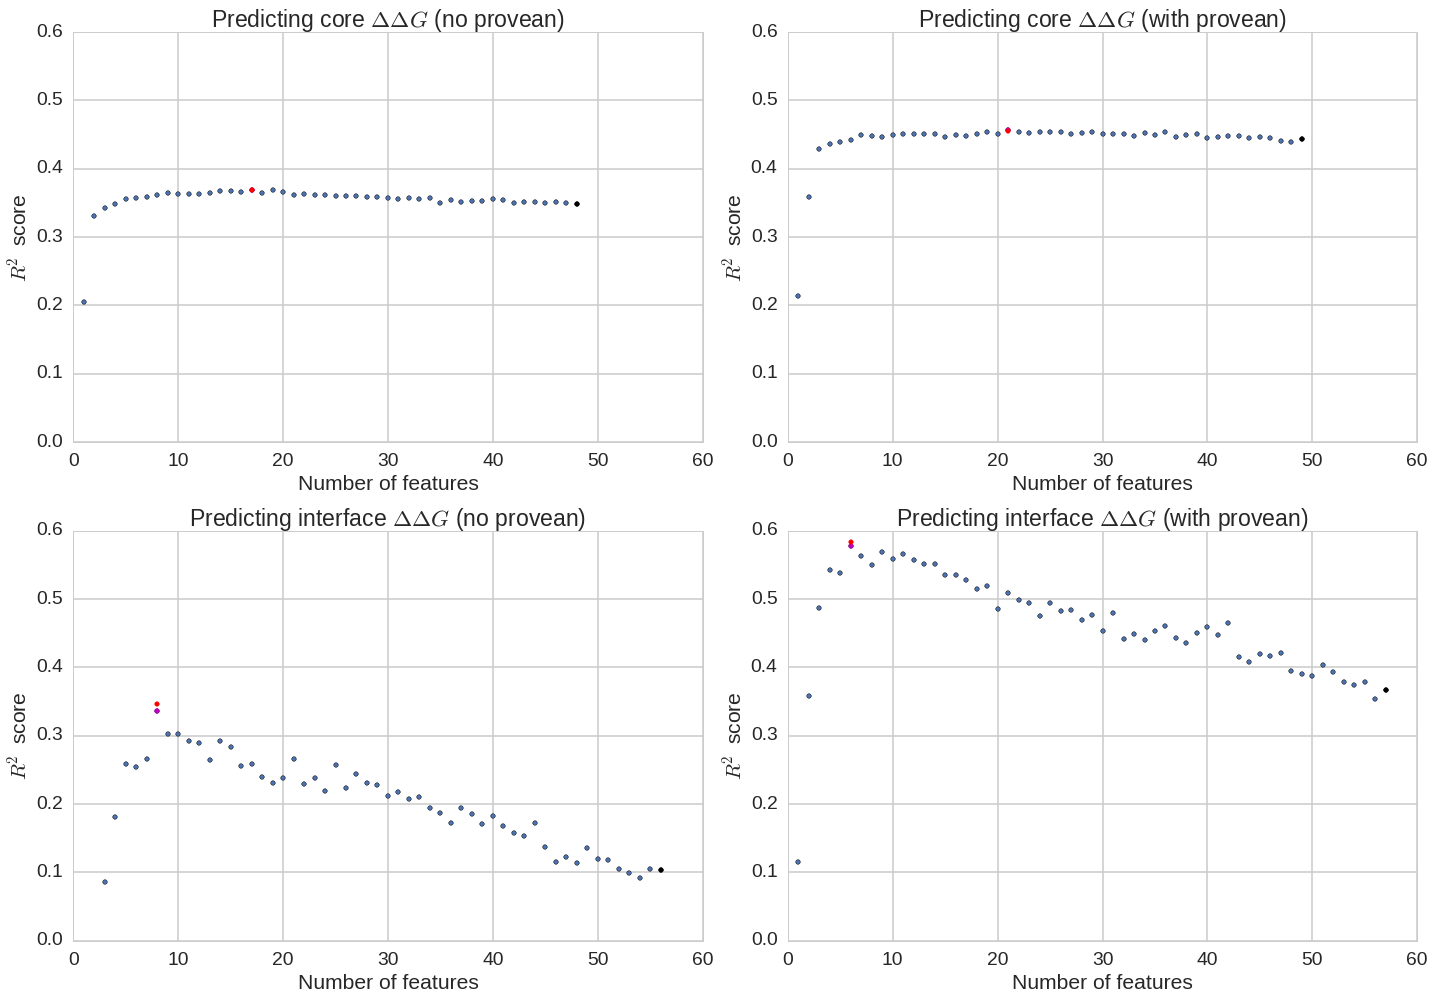
\includegraphics[scale=0.3]{image117}
	\caption{Variable elimination.}
\end{figure}

\begin{figure}[H]
	\centering
	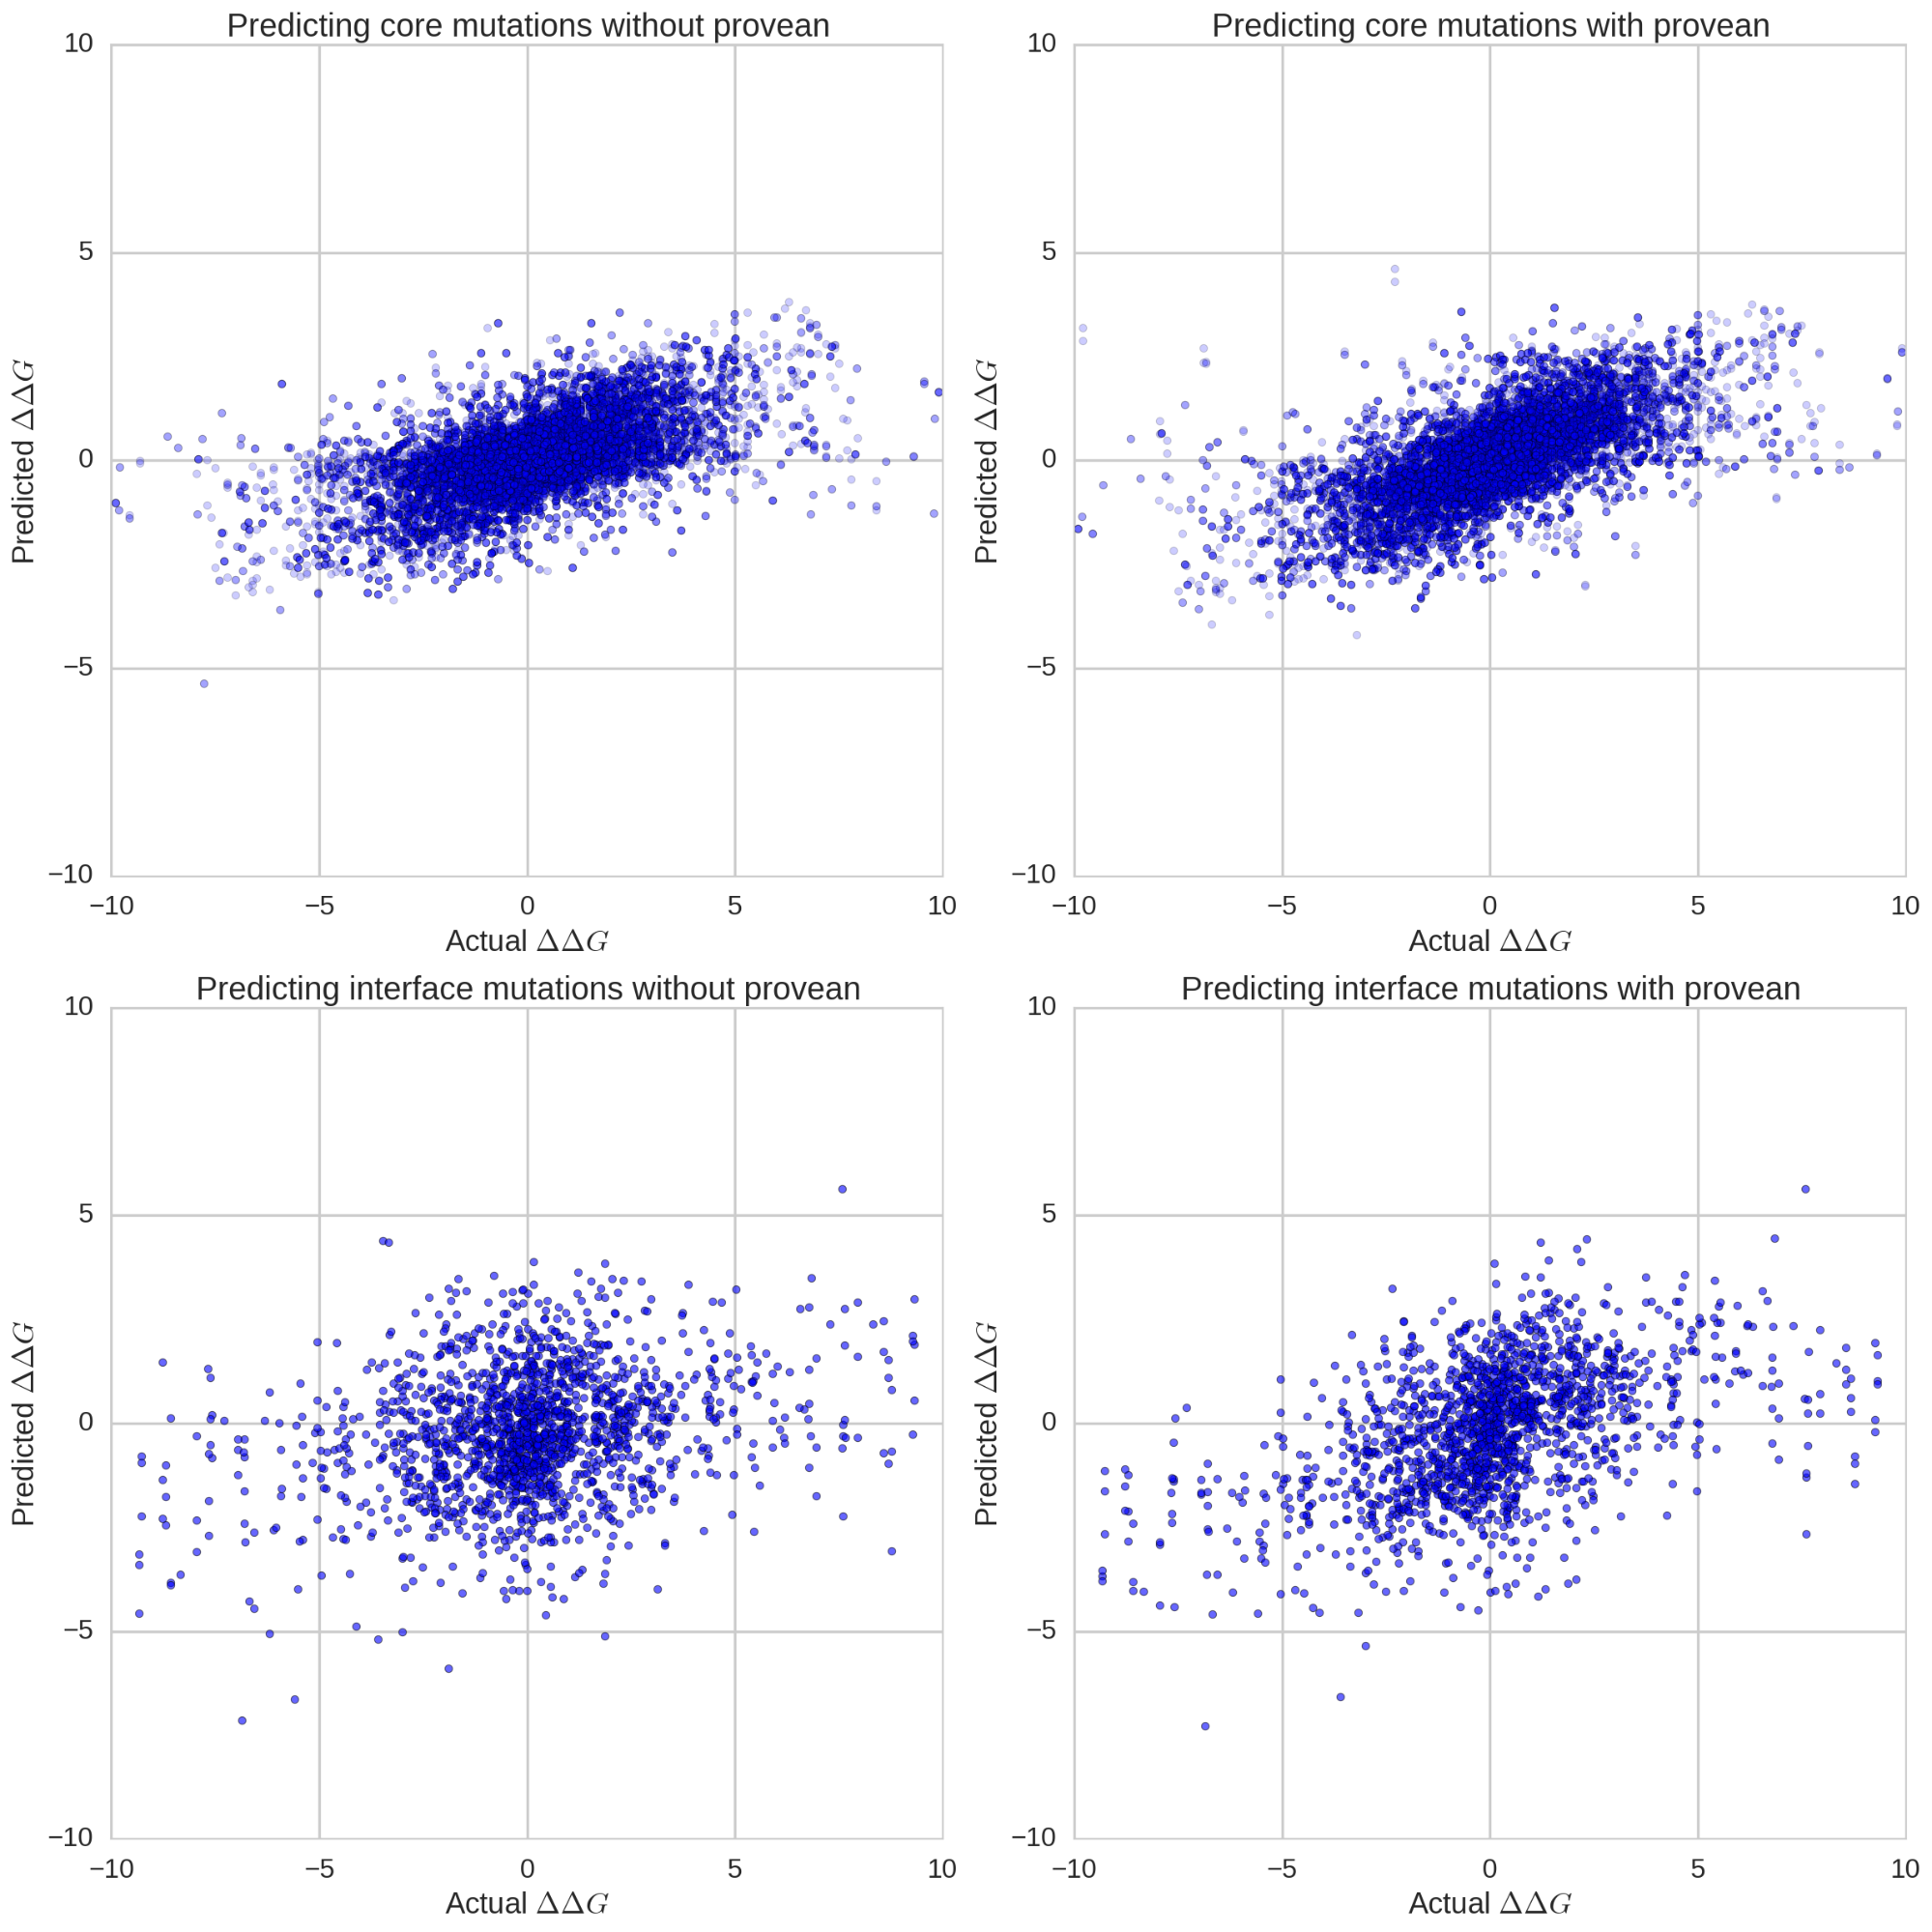
\includegraphics[scale=0.2]{image65}
	\caption{Cross-validation performance before variable elimination.}
\end{figure}

\begin{figure}[H]
	\centering
	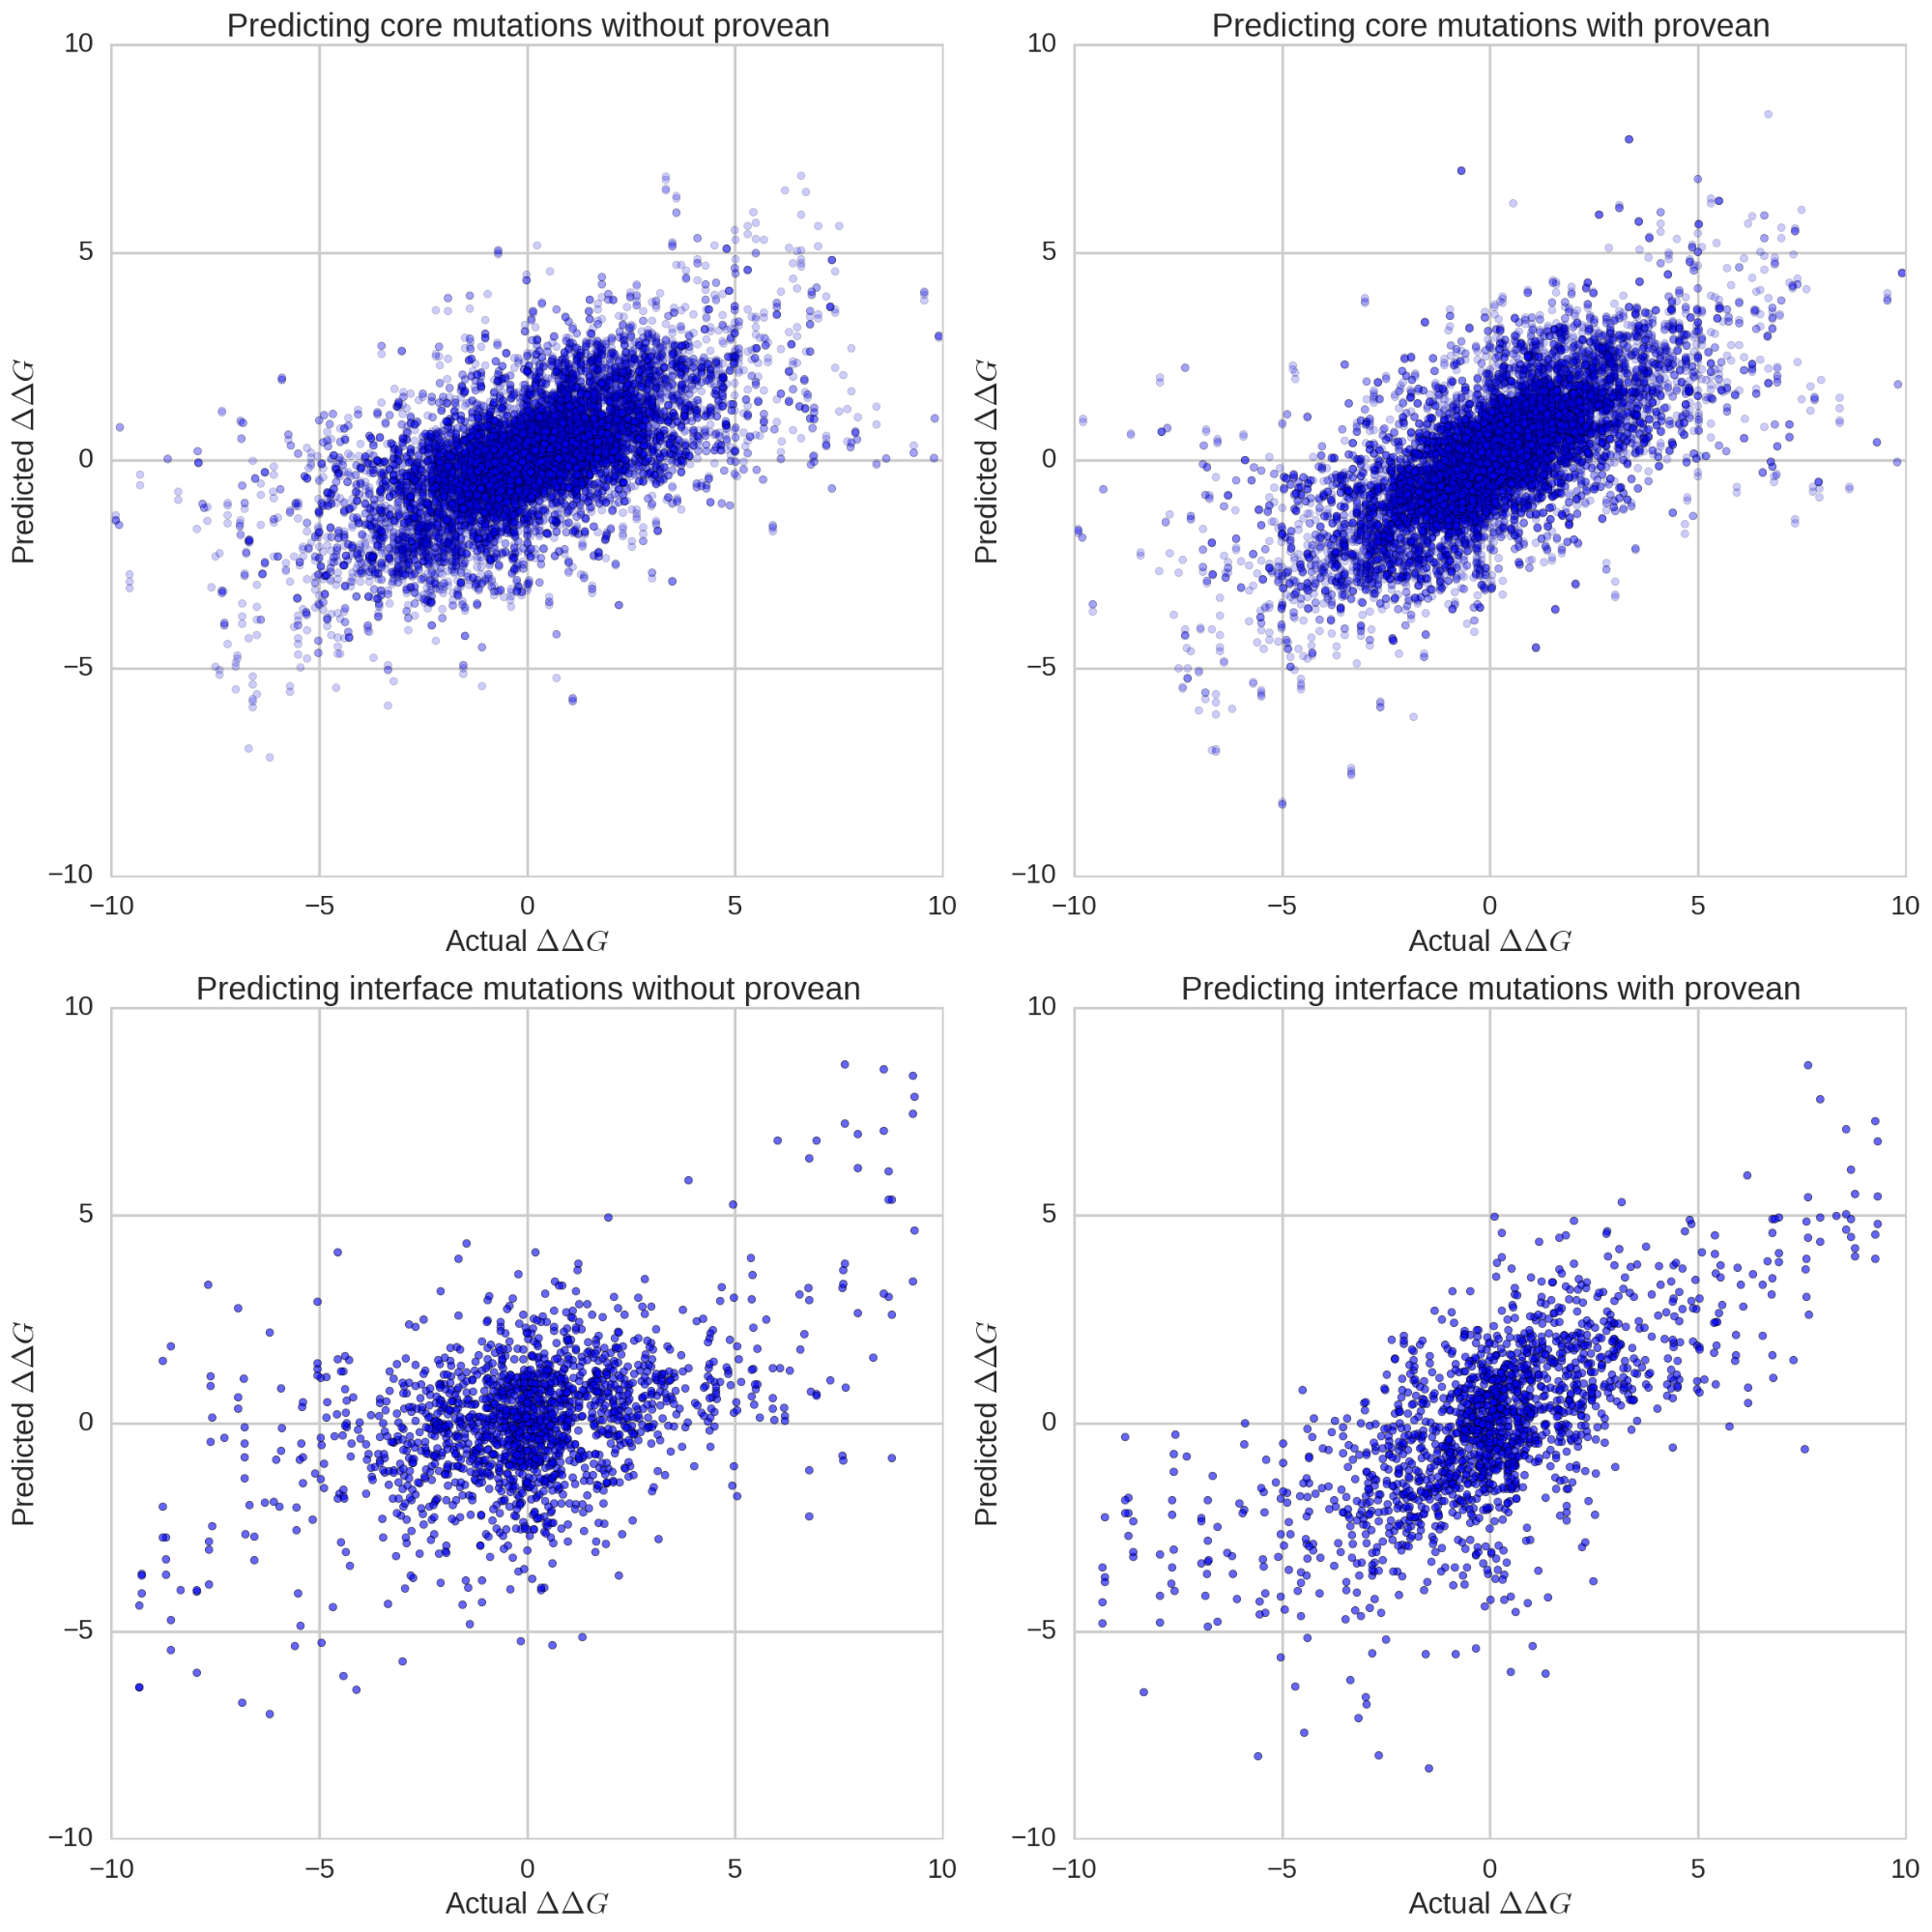
\includegraphics[scale=0.2]{image103}
	\caption{Cross-validation performance after variable elimination.}
\end{figure}

\begin{figure}[H]
	\centering
	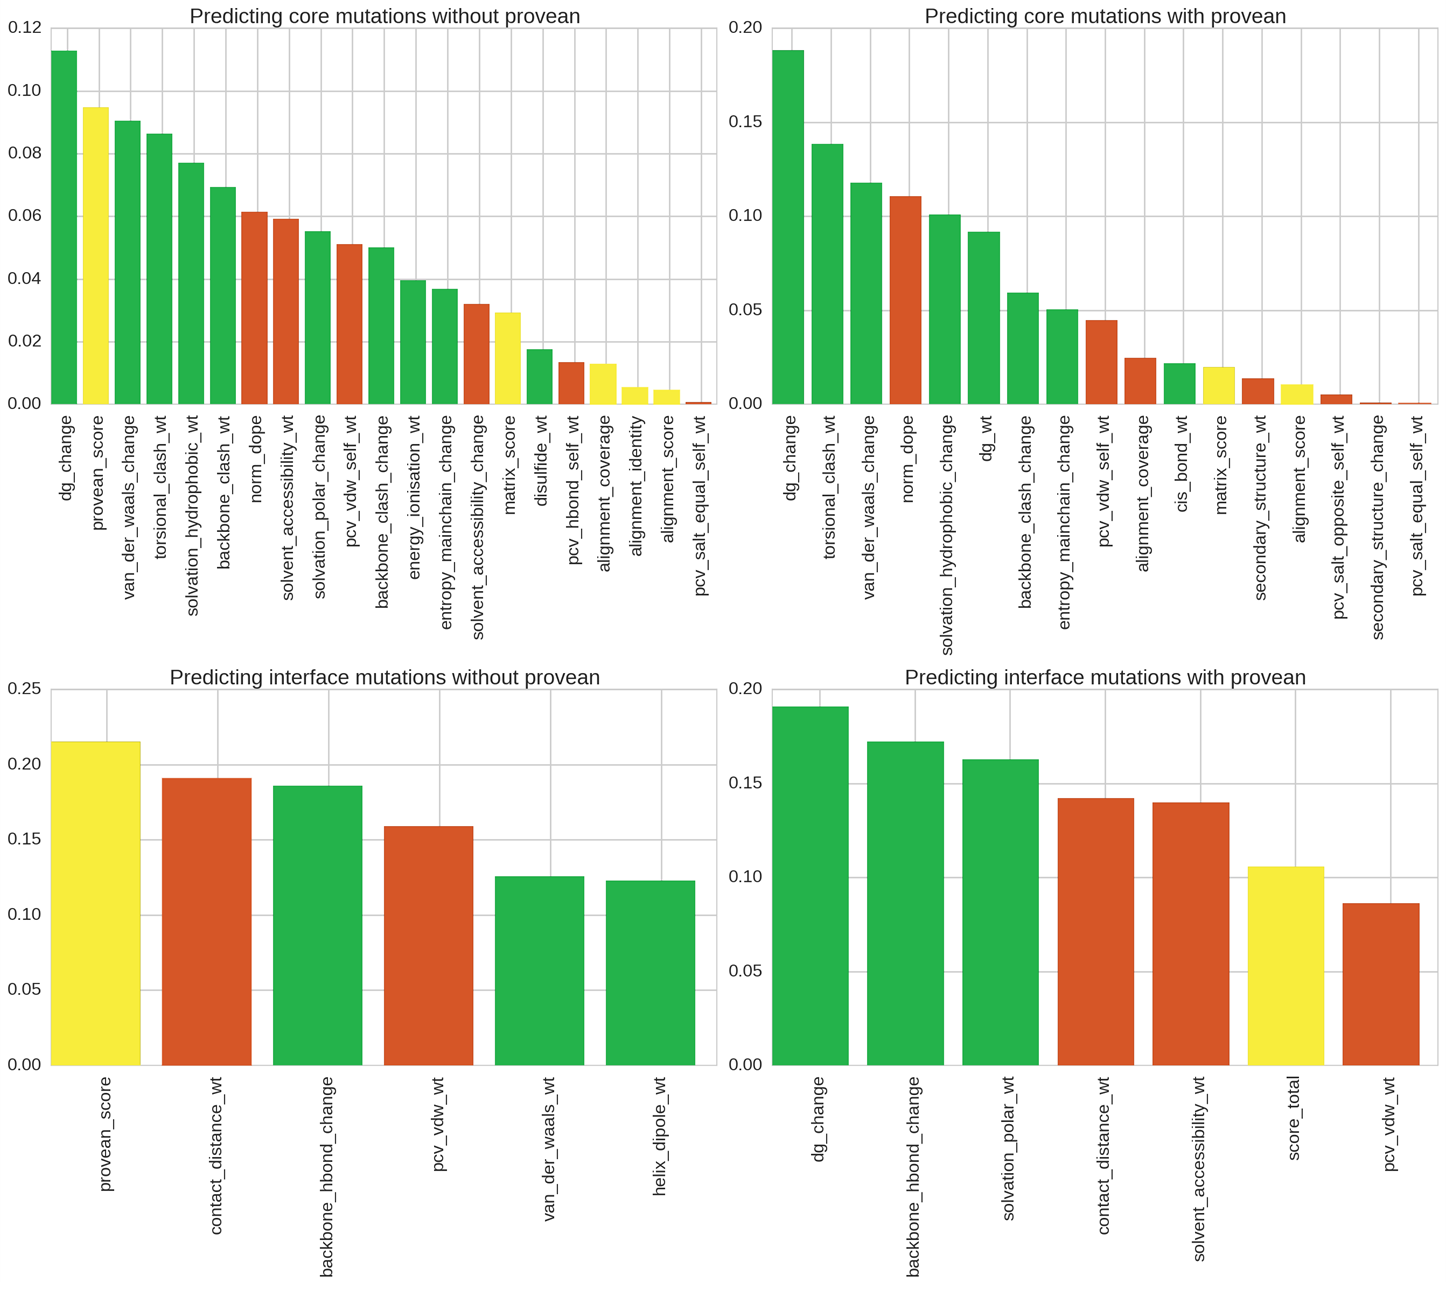
\includegraphics[scale=0.3]{image02}
	\caption{Feature importances after variable elimination.}
\end{figure}




\subsection{Validation}

Compare how well Provean, FoldX, and `ELASPIC with Provean' and `ELASPIC without Provean' distinguish between the three different datasets for both core and interface mutations.

\begin{itemize}
\item Chaperone interaction data (core mutations) \ Luciferase complementation assay (interface mutations) (use Spearman correlation coefficient).
\item Uniprot disease vs. polymorphism (use AUC / ROC / combination).
\item COSMIC driver vs. passenger.
\end{itemize}







\subsubsection{Chaperone interaction data}

\begin{figure}[H]
	\centering
	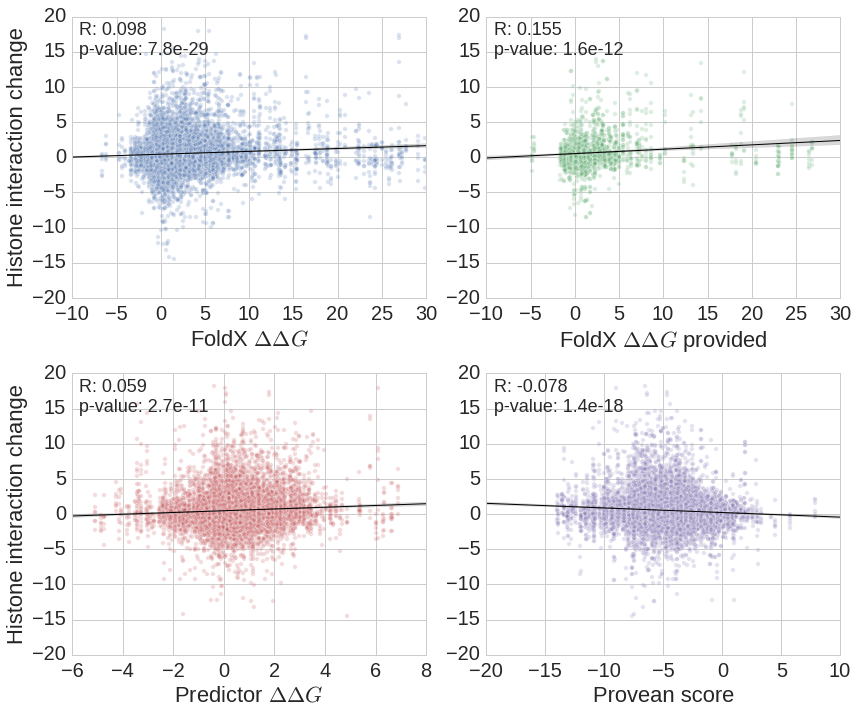
\includegraphics[scale=0.4]{image75}
	\caption[Core Validation]{Validation of the ELASPIC core predictor using chaperone interaction data from "Widespread Macromolecular Interaction Perturbations in Human Genetic Disorders".}
\end{figure}


\begin{figure}[H]
	\centering
	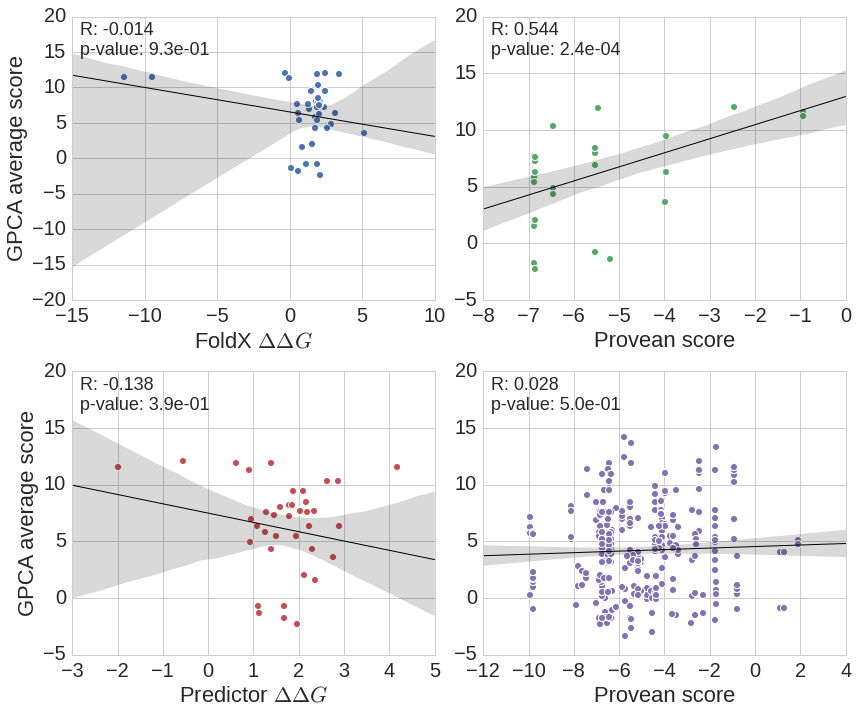
\includegraphics[scale=0.4]{image52}
	\caption[Interface Validation]{Validation of the ELASPIC core interface predictor using \textit{Gaussia princeps} luciferase protein complementation assay from "Widespread Macromolecular Interaction Perturbations in Human Genetic Disorders".}
\end{figure}









\section{Structure features}

The performance of Provean is comparable to the leading mutation scoring programs, such as SITF, PolyPhen-2, Mutation Assessor, and CONDEL \cite{choi_predicting_2012}. Furthermore, Provean is distributed under a GPLv3 license, and uses \textit{supporting sets} of at most 45 sequences which can precalculated and stored. If a supporting set is available, calculating the Provean score takes several seconds per mutation.

Another widely-used mutaiton scoring tool is PolyPhen-2. It is one of the packages predicted for






\section{ELASPIC pipeline}


xxx

\begin{figure}[H]
	\centering
	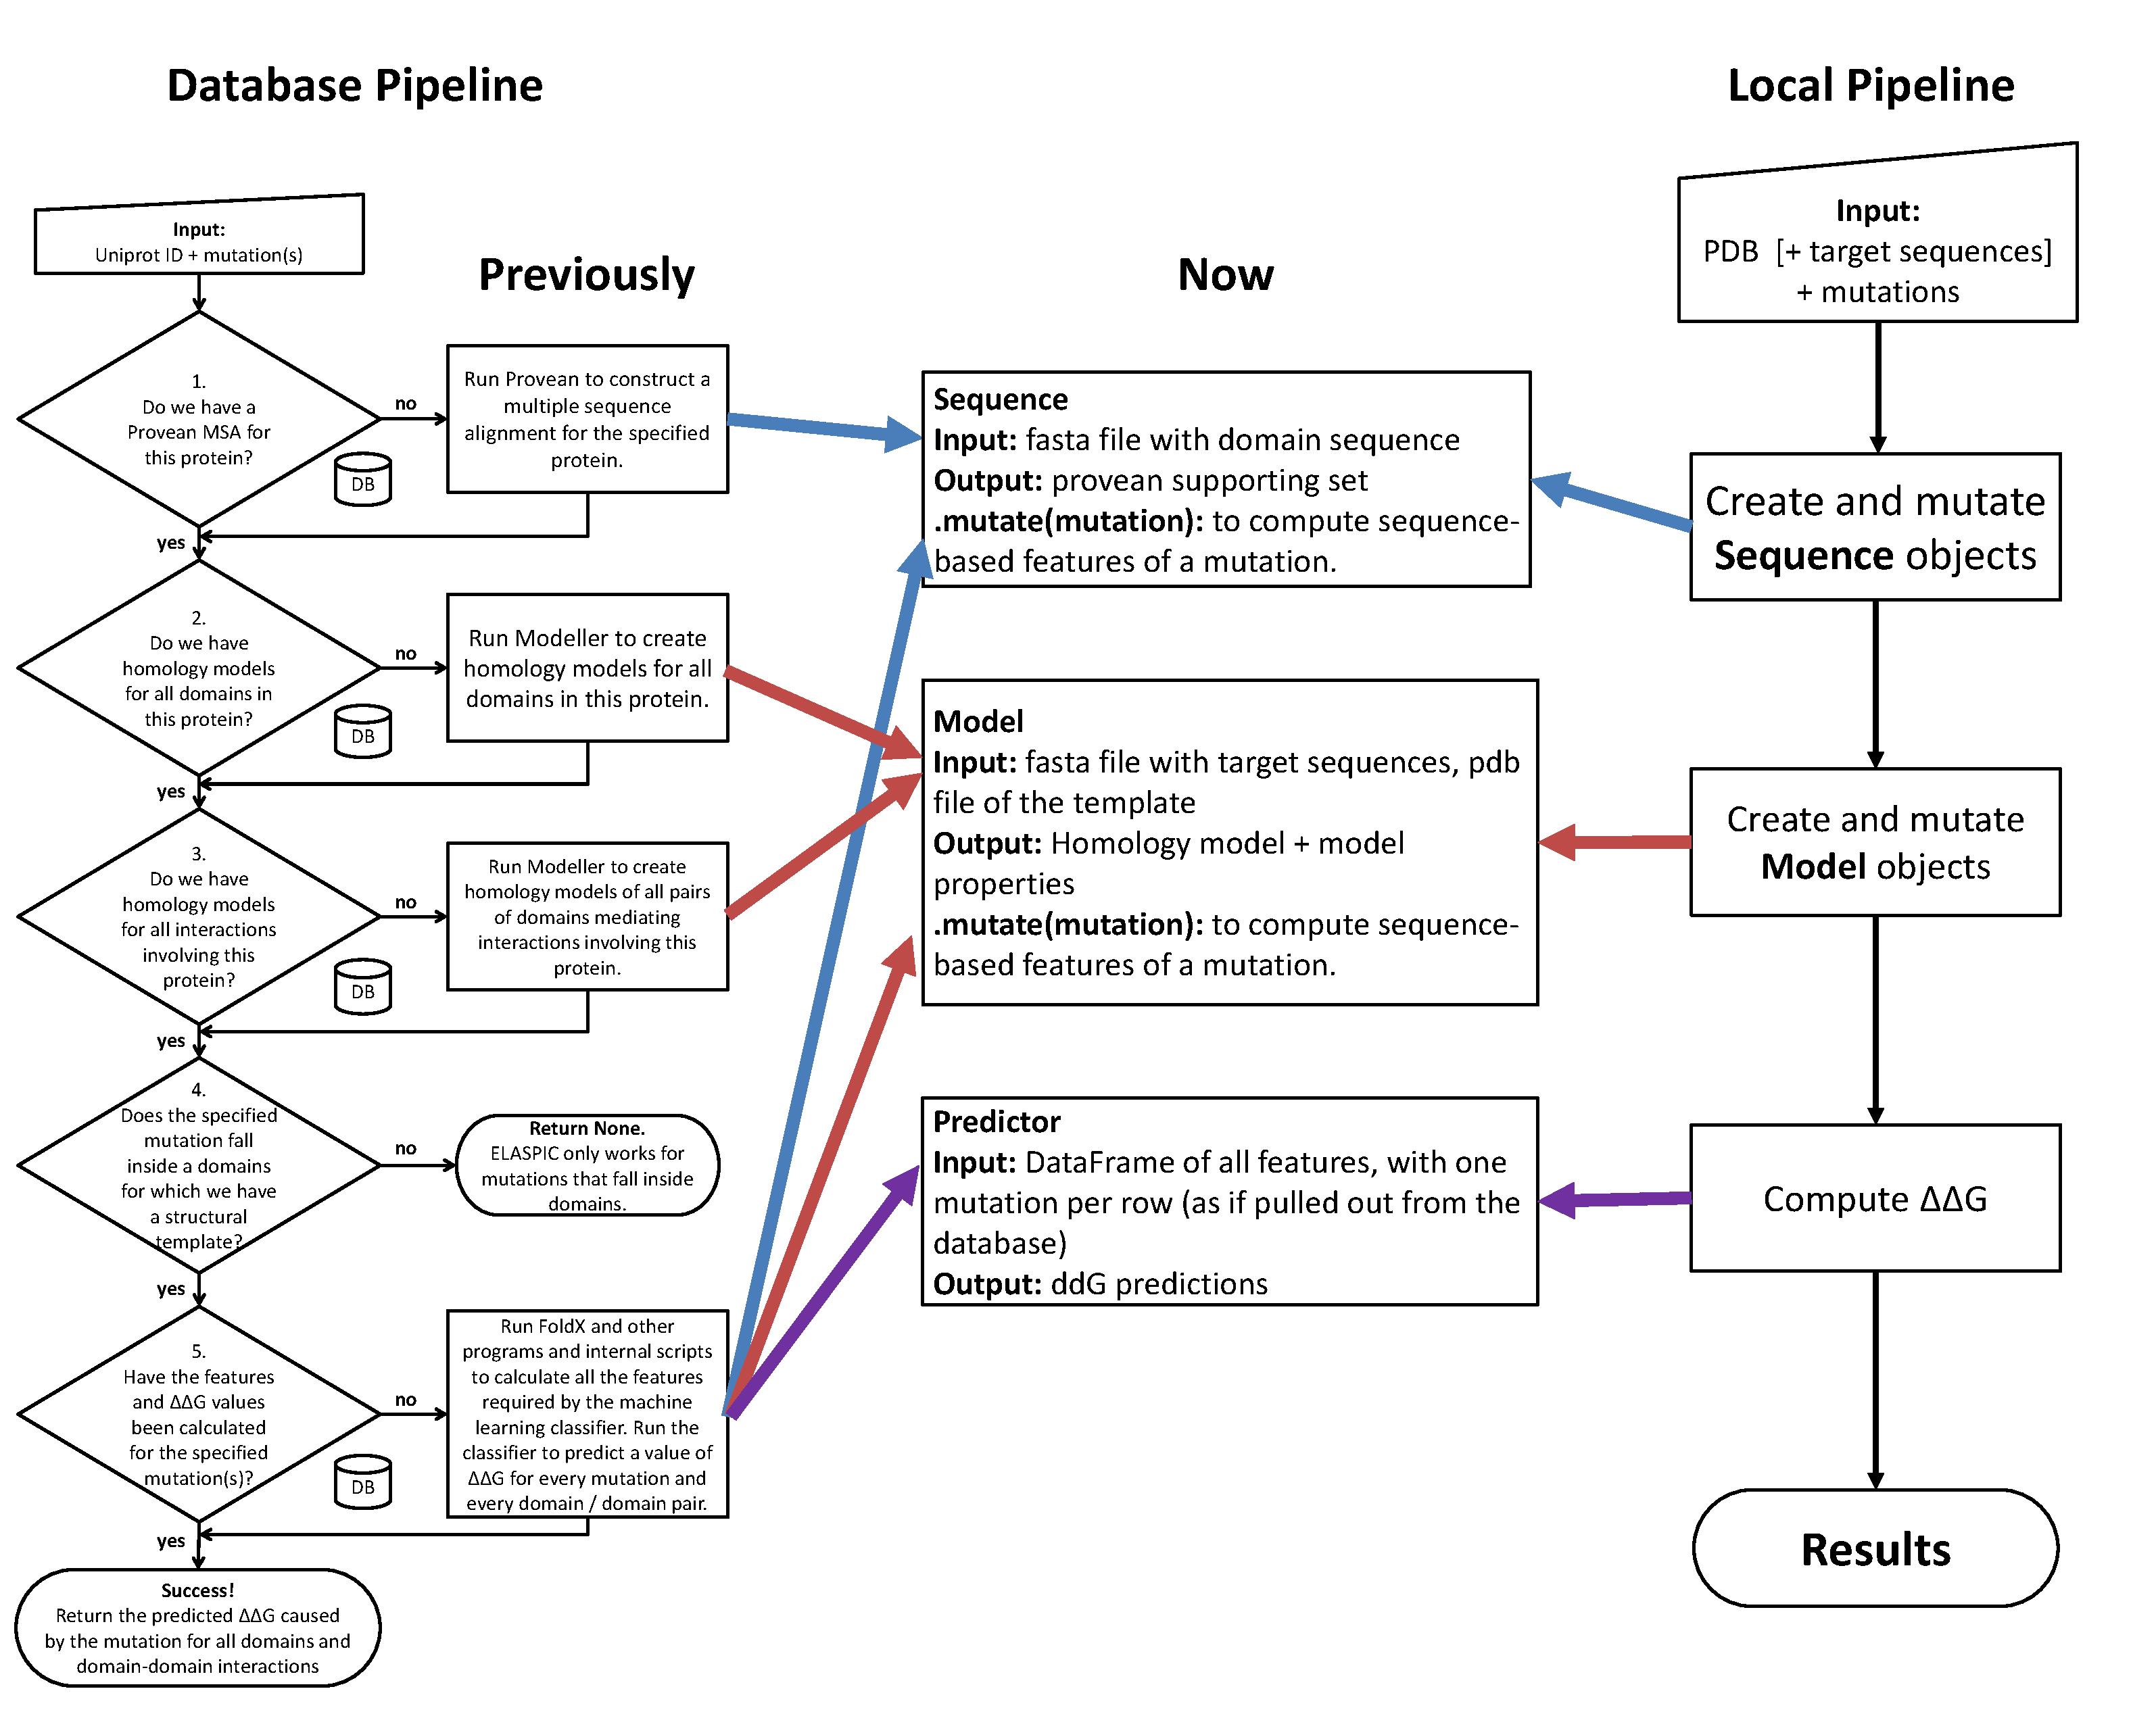
\includegraphics[scale=0.3]{diagrams_new.pdf}
	\caption[pipeline]{Pipeline of the ELASPIC web service.}
\end{figure}



\section{ELASPIC web service}

\begin{table}[H]
	\centering
	\caption{ELASPIC web service API.}
	\label{my-label}
	\begin{tabular}{lll}
	\textbf{Method} & \textbf{HTTP request} & \textbf{Description} \\
	submitjob & POST /submitjob & Submit a job to be run on a SGE cluser. \\
	jobstatus & GET /submitjob & View the results of a job.
	\end{tabular}
\end{table}
